\begin{frame}
	\frametitle{Chaos modelling. Different regimes.}
	
%	Unimodular, multimodular and chaotic regimes of laser work:	
	\begin{figure}
		\centering
		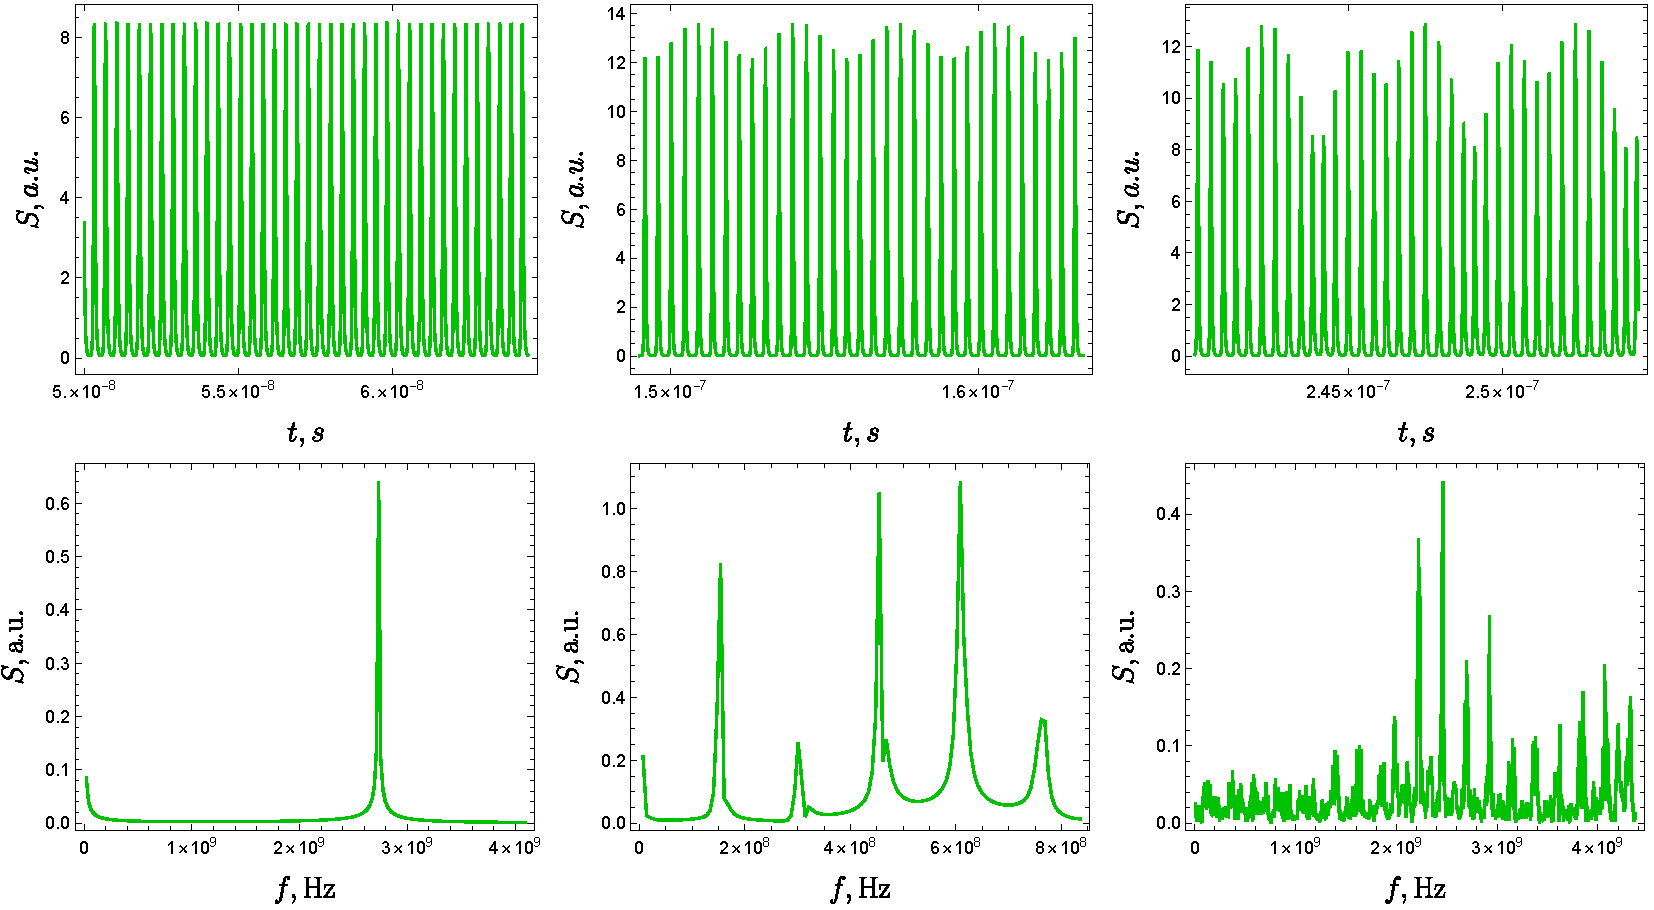
\includegraphics[width=\linewidth]{figures/chaos_and_spectra.pdf}
	\end{figure}
	
	\begin{center}
		\begin{tabular}{c|c|c|c}
			Delay time $\tau$ & $2 \ T_r$ & $7.5 \ T_r$ & $12 \ T_r$
		\end{tabular}
	\end{center}

%	Here dimensionless variable $s = \dfrac{S}{S_0}$.
	
	
\end{frame}	

\begin{frame}
	\frametitle{Chaos modelling.}
	Lyapunov exponents calculation :
	
	\begin{figure}
		\centering
		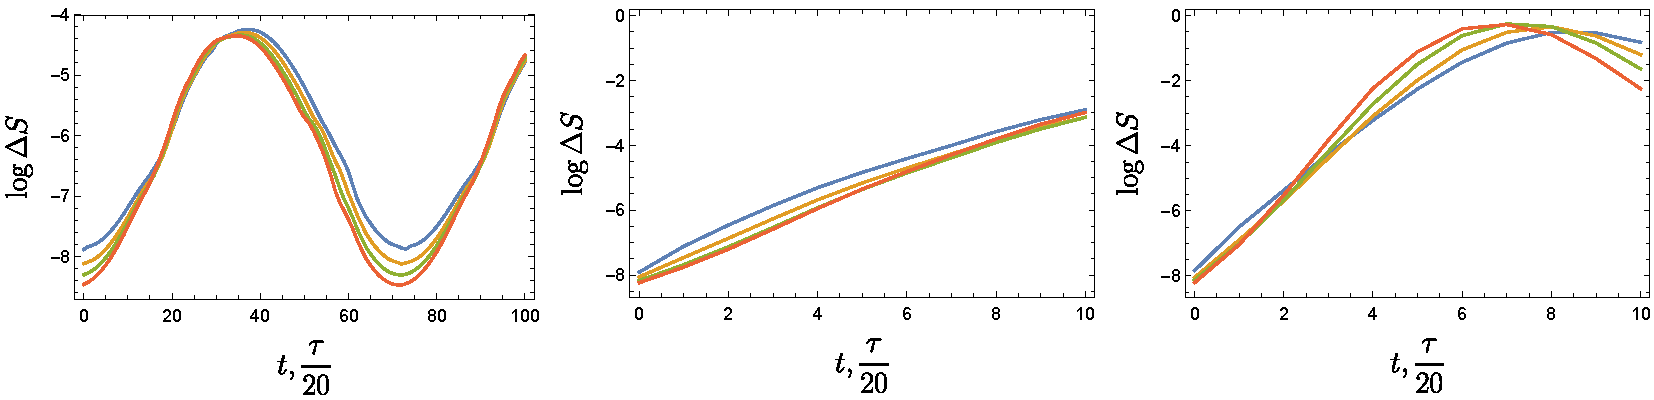
\includegraphics[width=\linewidth]{figures/lyapunovs.pdf}
	\end{figure}

\begin{columns}
	\begin{column}{0.4\linewidth}
		\begin{tabular}{c|c|c|c}
		$\tau$ & $2 \ T_r$ & $7.5 \ T_r$ & $12 \ T_r$	\\ \hline
		$\lambda$ & $0.0$ & $1.62 \ f_r$ & $1.84 \ f_r$
		\end{tabular}	
	\end{column}
	\begin{column}{0.6\linewidth}
		
		$\Delta S \sim \exp(\lambda t) \ \Rightarrow \ \log \Delta S = \lambda t + \const$\\[5pt]
		In real system $S_0^{-1} \int_{0}^{\infty} f(\eta) S(t-\eta)d\eta$ instead of $S(t-\tau)$. It reduces oscillations.
	\end{column}
\end{columns}	
\begin{center}
\end{center}
\end{frame}	
